% Compile with: latexmk -pdf proposal.tex
% Alternatively: tectonic proposal.tex
% Self-contained ACM proposal: figures are vector TikZ drawings and the
% bibliography is embedded. No separate images, .bib, or style files needed
% on Overleaf or a LaTeX installation with acmart and TikZ available.
% All experiment counts are planned quantities, not observed results.
\documentclass[sigconf,nonacm]{acmart}
\usepackage{array}
\usepackage{tikz}
\usetikzlibrary{arrows.meta,positioning,calc}
\setlength{\emergencystretch}{1em}
\definecolor{agentink}{HTML}{25475B}
\definecolor{agentfill}{HTML}{EDF3F6}
\definecolor{repairink}{HTML}{8A4D13}
\definecolor{repairfill}{HTML}{FAF1E5}
\definecolor{quietfill}{HTML}{F3F4F5}

\settopmatter{printacmref=false,printccs=false,printfolios=true}
\setcopyright{none}
\acmConference[CSE 5106]{CSE 5106: Multi-Agent Systems}{Fall 2026}{}
\acmYear{2026}

\title{Evidence-Checked Question Answering over FHIR Patient Records}
\subtitle{Multi-Agent Systems Project Proposal}
\author{Jeffrey Chen}
\affiliation{%
  \institution{Washington University in St. Louis}
  \city{St. Louis}
  \country{USA}
}
\author{Brant Yang}
\affiliation{%
  \institution{Washington University in St. Louis}
  \city{St. Louis}
  \country{USA}
}
\author{Akash Jairam}
\affiliation{%
  \institution{Washington University in St. Louis}
  \city{St. Louis}
  \country{USA}
}
\renewcommand{\shortauthors}{Chen, Yang, and Jairam}

\begin{document}

\begin{abstract}
We study factual questions about a patient's recorded history: for example, when a vital sign first crossed a threshold, or how many hospital admissions occurred. The evidence consists of structured FHIR records, and FHIR-AgentBench supplies questions and reference answers. Our system assigns retrieval, calculation, and verification to three LLM agents, with one targeted repair when evidence or reasoning is wrong. We compare it with a direct zero-shot LLM and a single agent using the same tools. A patient-disjoint evaluation will measure answer correctness, evidence validity, recovery from missing records, and computational cost.
\end{abstract}

\maketitle
\fancyhead{}

\section{Problem and Intended Task}
Answering a patient-record question requires finding the right encounter, selecting events in a time window, and sometimes calculating a result. An LLM may omit evidence, confuse measurement and posting times, or produce an incorrect total. We seek \textbf{correct, traceable answers about recorded care}, without diagnosing patients or recommending treatment.

Each task supplies a natural-language question, patient FHIR identifier, and reference-time assumptions. The output is a short answer with supporting resource IDs, field paths, and values, or an explicit evidence limitation. An empty result established from the record differs from failure to retrieve sufficient evidence.

\textbf{Research question.} Does separating retrieval, analysis, and record-based verification improve correctness and recovery beyond a direct LLM and a tool-equipped single agent, under comparable resource limits?

% Original vector figure. Design guidance consulted 2026-09-15:
% https://www.nature.com/documents/natrev-artworkguide_PS.pdf
% https://research-figure-guide.nature.com/figures/preparing-figures-our-specifications/
% Logical reading order, consistent encodings, limited semantic colour,
% editable vector text, and an explicit example of the proposed mechanism.
\begin{figure*}[!t]
\centering
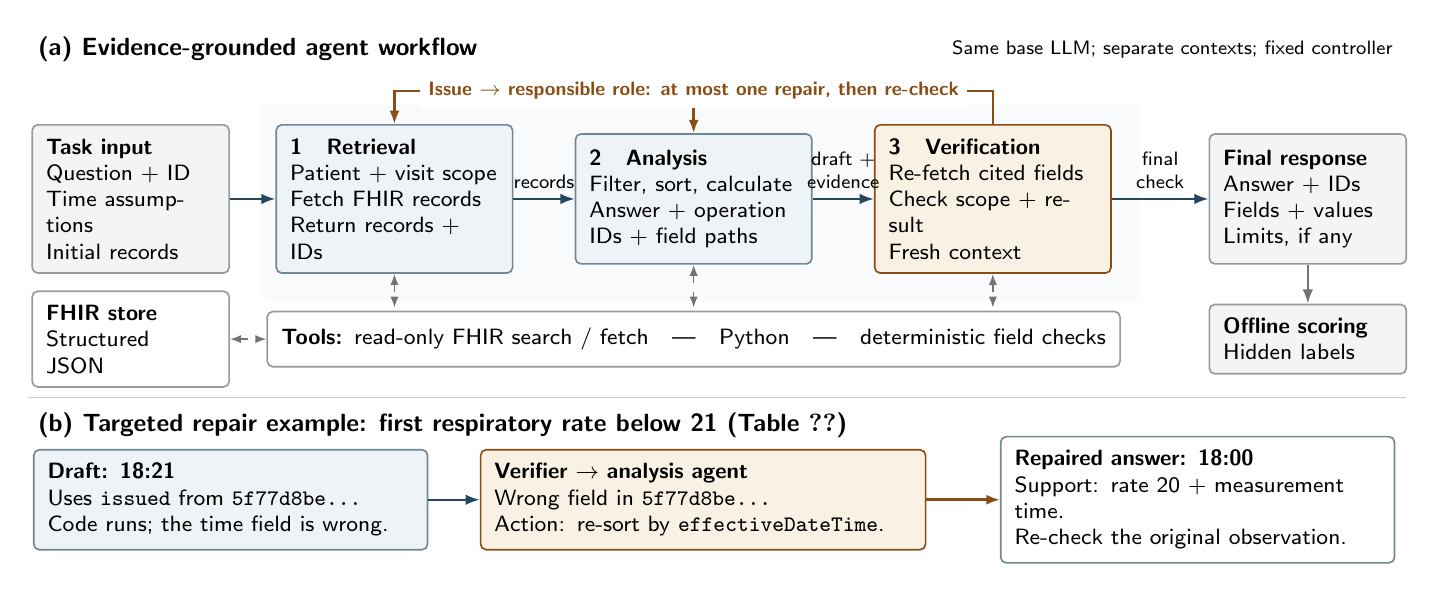
\begin{tikzpicture}[
  x=1cm,y=1cm,
  every node/.style={font=\sffamily\fontsize{8}{9.5}\selectfont},
  card/.style={draw=agentink!65,fill=white,rounded corners=2pt,
    line width=.6pt,align=left,inner sep=5pt},
  role/.style={card,text width=2.65cm,minimum height=1.65cm,fill=agentfill},
  terminal/.style={card,draw=black!40,fill=quietfill,text width=2.15cm,minimum height=1.65cm},
  flow/.style={-{Latex[length=1.8mm]},draw=agentink,line width=.8pt},
  access/.style={{Latex[length=1.4mm]}-{Latex[length=1.4mm]},draw=black!55,dashed,line width=.6pt},
  repair/.style={-{Latex[length=1.7mm]},draw=repairink,line width=.9pt},
  smalllabel/.style={font=\sffamily\fontsize{7.3}{8.5}\selectfont,align=center}
]
% (a) The only LLM instances are the three numbered roles.
\node[anchor=west,font=\sffamily\bfseries\fontsize{9}{11}\selectfont] at (0,5.55)
  {(a) Evidence-grounded agent workflow};
\node[anchor=east,smalllabel] at (17.45,5.55)
  {Same base LLM; separate contexts; fixed controller};
\fill[agentfill!40,rounded corners=3pt] (2.95,2.35) rectangle (14.12,4.85);
\node[terminal] (input) at (1.3,3.65)
  {\textbf{Task input}\\Question + ID\\Time assumptions\\Initial records};
\node[role] (retrieve) at (4.65,3.65)
  {\textbf{1\quad Retrieval}\\Patient + visit scope\\Fetch FHIR records\\Return records + IDs};
\node[role] (analyze) at (8.45,3.65)
  {\textbf{2\quad Analysis}\\Filter, sort, calculate\\Answer + operation\\IDs + field paths};
\node[role,draw=repairink,fill=repairfill] (verify) at (12.25,3.65)
  {\textbf{3\quad Verification}\\Re-fetch cited fields\\Check scope + result\\Fresh context};
\node[terminal] (answer) at (16.25,3.65)
  {\textbf{Final response}\\Answer + IDs\\Fields + values\\Limits, if any};
\draw[flow] (input.east) -- (retrieve.west);
\draw[flow] (retrieve.east) -- node[above,smalllabel] {records} (analyze.west);
\draw[flow] (analyze.east) -- node[above,smalllabel] {draft +\\evidence} (verify.west);
\draw[flow] (verify.east) -- node[above,smalllabel] {final\\check} (answer.west);
% A typed request returns only to the responsible role, at most once.
\draw[repair] (verify.north) -- (12.25,5.02) -- (4.65,5.02) -- (retrieve.north);
\draw[repair] (8.45,5.02) -- (analyze.north);
\node[smalllabel,fill=white,inner sep=3pt,text=repairink] at (8.45,5.02)
  {\textbf{Issue $\rightarrow$ responsible role: at most one repair, then re-check}};

% Tool access has a distinct line encoding; the store is unchanged by agents.
\node[card,text width=2.15cm,minimum height=.70cm,draw=black!40] (store) at (1.3,1.87)
  {\textbf{FHIR store}\\Structured JSON};
\node[card,text width=10.48cm,minimum height=.70cm,align=center,draw=black!40] (tools) at (8.45,1.87)
  {\textbf{Tools:} read-only FHIR search / fetch\quad |\quad Python\quad |\quad deterministic field checks};
\draw[access] (store.east) -- (tools.west);
\draw[access] (retrieve.south) -- (4.65,2.27);
\draw[access] (analyze.south) -- (8.45,2.27);
\draw[access] (verify.south) -- (12.25,2.27);
\node[card,text width=2.15cm,minimum height=.70cm,draw=black!40,fill=quietfill] (eval) at (16.25,1.87)
  {\textbf{Offline scoring}\\Hidden labels};
\draw[flow,draw=black!55] (answer.south) -- (eval.north);
% (b) A worked semantic error, not an invented experimental result.
\draw[black!20,line width=.45pt] (0,1.13) -- (17.5,1.13);
\node[anchor=west,font=\sffamily\bfseries\fontsize{9}{11}\selectfont] at (0,.78)
  {(b) Targeted repair example: first respiratory rate below 21 (Table~\ref{tab:example})};
\node[card,text width=4.65cm,minimum height=1.02cm,fill=agentfill] (draft) at (2.57,-.17)
  {\textbf{Draft: 18:21}\\Uses \texttt{issued} from \texttt{5f77d8be\ldots}\\Code runs; the time field is wrong.};
\node[card,text width=5.3cm,minimum height=1.02cm,draw=repairink,fill=repairfill] (issue) at (8.57,-.17)
  {\textbf{Verifier $\rightarrow$ analysis agent}\\Wrong field in \texttt{5f77d8be\ldots}\\Action: re-sort by \texttt{effectiveDateTime}.};
\node[card,text width=4.65cm,minimum height=1.02cm] (fixed) at (14.85,-.17)
  {\textbf{Repaired answer: 18:00}\\Support: rate 20 + measurement time.\\Re-check the original observation.};
\draw[flow] (draft.east) -- (issue.west);
\draw[repair] (issue.east) -- (fixed.west);
\end{tikzpicture}
\caption{Proposed workflow and a worked repair. Solid arrows carry outputs, amber arrows route errors, and dashed arrows denote tool access. The verifier checks original records without the analyst's reasoning history; only offline scoring sees gold labels.}
\Description{Panel a shows retrieval, analysis, and verification roles using shared tools over an unchanged FHIR store, followed by an evidence-linked response and separate offline scoring. A verifier can request one targeted repair. Panel b illustrates correcting a posting-time error by selecting the observation's measurement-time field.}
\label{fig:architecture}
\end{figure*}

\section{Related Work}
Recent EHR question answering increasingly uses executable retrieval and reasoning. EHRAgent (2024) translates multi-table clinical questions into code and improves programs using execution feedback~\cite{shi2024}. FHIR-AgentBench (2026) extends evaluation to interoperable FHIR resources and separates retrieval choices from language- and code-based reasoning~\cite{lee2026}. FHIRPath-QA (2026) instead generates executable FHIRPath queries, showing how explicit operations can reduce dependence on free-text reasoning~\cite{frew2026}. These studies motivate structured evidence and executable calculations; our question is whether separate verification improves answers after execution succeeds.

A parallel direction distributes medical reasoning across roles. MedAgents (2024) coordinates expert-style analyses and discussion on medical knowledge benchmarks~\cite{tang2024}; these tasks differ from retrieving a particular patient's records. EHRNavigator (2026) brings specialization to patient-level QA, coordinating structured queries, clinical-note retrieval, and answer synthesis~\cite{qian2026}. It is our closest architectural precedent: its SQL revision loop addresses execution failures. We test field-level errors even when execution succeeds. Multi-agent EHR QA itself is already established.

Verification research suggests both opportunities and limits. Chain-of-Verification (2024) reduces dependence on an initial response by answering verification questions independently~\cite{dhuliawala2024}; CRITIC (2024) uses external tools to critique and revise outputs~\cite{gou2024}. MAST (2025) identifies coordination and verification failures across multi-agent systems~\cite{cemri2025}, cautioning that extra roles alone do not ensure better results. These findings motivate fresh-context, source-grounded checks, structured error messages, and a bounded repair loop. Our course-level extension combines \textbf{field-linked verification and targeted repair} with a controlled missing-evidence test against a capable single agent. We will reuse FHIR-AgentBench's \textbf{single-agent baselines} and tools, and an existing agent framework for execution/message passing; we implement the team protocol ourselves. We evaluate the combined design.

\section{Data and Question Types}
We use the public MIMIC-IV Clinical Database Demo on FHIR v2.1.0: deidentified records for 100 patients~\cite{mimicdemo}. FHIR (Fast Healthcare Interoperability Resources) represents information as linked JSON resources, distributed here as gzip-compressed \emph{newline-delimited JSON}. The modality is \textbf{structured clinical data}: categorical codes, numerical measurements, timestamps, and record references; images, audio, and external literature are excluded.

Each \texttt{Observation} links to a \texttt{Patient} and an \texttt{Encounter} (visit). It contains a value/unit (\texttt{valueQuantity}), measurement time (\texttt{effectiveDateTime}), and issue time (\texttt{issued}). Table~\ref{tab:example} presents actual records as rows.

\begin{table}[!t]
\caption{Real respiratory-rate observations for patient 10015860 on 2186-09-15 (UTC offset $-04{:}00$). Selected rows from the patient history; IDs are abbreviated.}
\label{tab:example}
\centering
\small
\setlength{\tabcolsep}{4pt}
\begin{tabular}{@{}lccc@{}}
\toprule
Observation ID & Measured & Issued & Rate (insp/min) \\
\midrule
\texttt{5f77d8be\ldots} & 18:00 & 18:21 & 20 \\
\texttt{a4b71266\ldots} & 18:21 & 18:22 & 18 \\
\texttt{e3bc23cf\ldots} & 19:00 & 19:06 & 21 \\
\bottomrule
\end{tabular}
\par\smallskip
\begin{minipage}{\columnwidth}
\small
\textbf{Query (paraphrased):} Since June 6, 2186, when did this patient's respiratory rate first fall below 21?\\
\textbf{Assumption:} Current time is 2186-12-31 23:59. Dates are shifted for deidentification.\\
\textbf{Reference answer:} 2186-09-15 18:00:00.\\
\textbf{Expected evidence:} \texttt{Observation/5f77d8be\ldots}, value 20, and its measurement timestamp. Using the \emph{issued} time would incorrectly answer 18:21; a value of 21 does not satisfy ``below 21.''
\end{minipage}
\end{table}
% Verified example: question_id 672d81cda5b780896726e4f2.
% patient_fhir_id: 1cf9e585-806c-513b-80af-4ca565a28231.
% Full source IDs: 5f77d8be-c363-502c-8031-b0e3b96ace3c,
% a4b71266-da9d-56b7-af91-603d724e9b69,
% e3bc23cf-cd3f-5367-a71b-fb933a4dbe90.
% Source: MIMIC-IV FHIR demo 2.1.0, fhir/MimicObservationChartevents.ndjson.gz.
% QA CSV inspected 2026-09-14; SHA256:
% e2045692fef7f5f4f77496935160f5fc727e162d213e94feed61401948e512a0

\textbf{Questions and labels.} FHIR-AgentBench~\cite{lee2026} supplies 2,931 questions in its \href{https://github.com/glee4810/FHIR-AgentBench/blob/master/final_dataset/questions_answers_sql_fhir.csv}{released QA CSV}, covering 94 of the demo's patients. Each row supplies the question, patient FHIR ID, and reference-time assumption. Reference answers (\texttt{true\_answer}), resource annotations (\texttt{true\_fhir\_ids}), SQL queries, and template metadata are hidden from agents. We select three question families:
\begin{itemize}
  \item \textbf{Lookup and counting:} e.g., count patient 10001217's hospital admissions (reference: 2).
  \item \textbf{Temporal selection:} first/last qualifying event within a date range, as in Table~\ref{tab:example}.
  \item \textbf{Numerical aggregation:} e.g., maximum prothrombin time (PT) during patient 10004235's latest hospital encounter (reference: 12.3).
\end{itemize}
Examples paraphrase released questions. We retain empty-answer cases; the three illustrated patients are reserved for development.

\section{Proposed Architecture}
Figure~\ref{fig:architecture} separates three responsibilities using \textbf{the same base LLM in three contexts}. A fixed controller shares the question and assumptions, routes structured messages, and limits repairs; it is not a fourth LLM.

\textbf{Retrieve.} The retrieval agent selects resource types, resolves patient/encounter scope, and searches the FHIR store. Separating evidence acquisition addresses the retrieval bottleneck documented by FHIR-AgentBench~\cite{lee2026}.

\textbf{Analyze.} The analysis agent filters and orders records and executes counts or arithmetic in Python. It returns a draft with resource IDs, field paths, and values; aggregates also record the operation and contributing IDs. This makes calculations inspectable, following the executable-reasoning direction of EHRAgent and FHIRPath-QA~\cite{shi2024,frew2026}.

\textbf{Verify and repair.} The verifier receives the draft/evidence without the analyst's reasoning history. It re-fetches original fields, checks patient/time/encounter scope, recomputes results, and searches again if completeness is doubtful. This combines reduced exposure to earlier reasoning~\cite{dhuliawala2024} with external tool feedback~\cite{gou2024}. A failed check yields \emph{issue type, record/field, responsible role, corrective action}. Missing evidence returns to retrieval; wrong fields or calculations return to analysis. After at most one repair cycle, the verifier re-checks and releases an answer or limitation. Figure~\ref{fig:architecture}(b) illustrates a semantic error that successful code execution alone cannot detect. Shared-model errors and harmful revisions remain possible and will be measured.

\section{Comparisons and Evaluation}
\subsection{Baselines and Budget Controls}
The systems in Table~\ref{tab:systems} receive the same question, assumptions, and starting packet. A deterministic retriever ranks resource labels by question keywords within the patient record and includes linked encounter metadata. Ranking and token truncation are fixed on development data without gold answers or IDs.

\begin{table}[!t]
\caption{Three systems using the same base LLM and answer/evidence format. The direct baseline is zero-shot.}
\label{tab:systems}
\centering
\small
\setlength{\tabcolsep}{3pt}
\begin{tabular}{@{}>{\raggedright\arraybackslash}p{.24\columnwidth}>{\raggedright\arraybackslash}p{.71\columnwidth}@{}}
\toprule
System & What it does \\
\midrule
\textbf{Direct LLM}\newline Zero-shot & Reads question + starting records and generates one answer. No live tools or revision. \\
\addlinespace[3pt]
\textbf{Single agent}\newline With tools & One LLM context searches the store, runs Python, checks evidence, and may revise once. \\
\addlinespace[3pt]
\textbf{Verified team}\newline Proposed system & Separate retrieval, analysis, and verification contexts exchange evidence and allow one targeted repair (Figure~\ref{fig:architecture}). \\
\bottomrule
\end{tabular}
\end{table}

The direct LLM measures improvement over simple prompting. The stronger single agent shares the team's store, retrieval/Python tools, deterministic field checks, and one-revision allowance, separating coordination benefits from tool access. We fix equal aggregate token and tool-call ceilings on development data and report actual usage, including repeated context.

\subsection{Answer and Evidence Scoring}
The primary measure is \textbf{typed answer accuracy} against hidden \texttt{true\_answer}: normalized numbers, timestamps at requested precision, categories, or sets. We fix tolerances/time normalization on development data and check claimed units. The \href{https://github.com/glee4810/FHIR-AgentBench/blob/master/evaluation_metrics.py}{official LLM-judge score} provides comparability but uses permissive numeric/date rules.

Evidence scoring resolves cited IDs and field paths against original records and checks values, units, timestamps, and encounter links. We report valid-evidence fraction and retrieval precision/recall against \texttt{true\_fhir\_ids}; these annotations can omit supporting dependencies, so overlap is diagnostic, not proof of completeness. Two teammates, blinded to system identity, audit 30--50 stratified outputs and scorer disagreements. We track unsupported claims, wrong-to-right repairs, right-to-wrong revisions, empty-answer correctness, tokens, and latency. Abstention is incorrect when the reference contains an answer.

\subsection{Experiment Size and Missing-Evidence Test}
A 20-question pilot and roughly 50 development questions precede 300 held-out questions spanning the three families. Because released splits overlap patients, we create a \textbf{patient-disjoint split} before testing. This is a subset study, not the official full-benchmark result. Paired comparisons use 95\% bootstrap intervals clustered by patient; a small fixed subset is repeated to assess run variability.

For 50 eligible held-out questions, both tool-enabled systems receive intact and perturbed starting packets. The harness removes one resource whose omission changes the answer derivable from the packet, excluding redundant-evidence cases. The original store remains intact; agents receive no omitted ID or missing-item marker and can recover evidence by searching. Gold labels are used only by the diagnostic harness. We measure the accuracy drop and omitted-resource recovery rate; the direct LLM is excluded because it cannot search.

The core plan is \textbf{900 ordinary runs} ($300\times3$ systems) plus \textbf{200 recovery runs} ($50\times2$ packet conditions $\times2$ systems): \textbf{1,100 runs for one model}, excluding development and selected repeats.

\section{Anticipated Results}
\textbf{Answer correctness.} We expect the largest improvements on temporal selection and aggregation, where mistakes can be checked against explicit fields and operations. Both tool-enabled systems should outperform direct prompting on these questions. The stronger hypothesis is that the verified team will also improve on the single agent by detecting wrong encounter scopes, timestamp fields, and incomplete evidence. On simple lookups with sufficient initial evidence, we expect little difference. These are hypotheses, not measured results.

\textbf{Evidence recovery.} The omission experiment should expose whether verification actively restores missing evidence. Support would mean a smaller accuracy drop and higher omitted-resource recovery for the team. We will inspect whether additional searches actually produce corrected answers: retrieving the omitted record without using it correctly is not successful recovery. Likewise, more valid citations without better answer accuracy would establish improved traceability, but not improved task performance.

\textbf{Efficiency and limits.} Extra verification should add cost and latency. Results will show accuracy by question family with paired confidence intervals, intact-versus-omitted accuracy, and helpful versus harmful revisions. An accuracy-versus-token-cost plot and median/95th-percentile latency will show whether any gain justifies coordination overhead. Higher cost with negligible improvement would favor the single agent for this task; intervals spanning zero would leave the advantage inconclusive. The small patient cohort and templated questions limit generalization, so we will not infer clinical effectiveness.

\section{Project Plan}
For three students over twelve weeks: weeks 1--4 establish data, scoring, and baselines; weeks 5--8 implement coordination and omissions; weeks 9--10 run experiments and build the demo; weeks 11--12 audit and report. After backend validation, an interface will support patient selection, example/custom questions, and inspection of answers, cited fields, and verification status. Its format remains open; queries use the evaluated backend and conversational follow-ups are deferred. Deliverables are code, split/perturbation manifests, results, and the demo. Extra models/ablations are optional. Training, clinician studies, literature synthesis, and the companion project's context construction are outside scope.

\begin{thebibliography}{9}

\bibitem[Shi et~al.(2024)]{shi2024}
Wenqi Shi et~al. 2024.
EHRAgent: Code Empowers Large Language Models for Few-shot Complex Tabular Reasoning on Electronic Health Records.
In \emph{EMNLP}, 22315--22339.
\url{https://doi.org/10.18653/v1/2024.emnlp-main.1245}

\bibitem[Lee et~al.(2026)]{lee2026}
Gyubok Lee et~al. 2026.
FHIR-AgentBench: Benchmarking LLM Agents for Realistic Interoperable EHR Question Answering.
In \emph{Machine Learning for Health}, PMLR 297, 1297--1315.
\url{https://proceedings.mlr.press/v297/lee26a.html}

\bibitem[Frew et~al.(2026)]{frew2026}
Michael Frew, Nishit Bheda, and Bryan Tripp. 2026.
FHIRPath-QA: Executable Question Answering over FHIR Electronic Health Records.
In \emph{CL4Health at LREC}, 1--14.
\url{https://doi.org/10.63317/5q8qi6jqnz56}

\bibitem[Tang et~al.(2024)]{tang2024}
Xiangru Tang et~al. 2024.
MedAgents: Large Language Models as Collaborators for Zero-shot Medical Reasoning.
In \emph{Findings of ACL}, 599--621.
\url{https://doi.org/10.18653/v1/2024.findings-acl.33}

\bibitem[Qian et~al.(2026)]{qian2026}
Lingfei Qian et~al. 2026.
EHRNavigator: A Multi-Agent System for Patient-Level Clinical Question Answering over Heterogeneous Electronic Health Records.
\emph{arXiv:2601.10020}.
\url{https://arxiv.org/abs/2601.10020}

\bibitem[Dhuliawala et~al.(2024)]{dhuliawala2024}
Shehzaad Dhuliawala et~al. 2024.
Chain-of-Verification Reduces Hallucination in Large Language Models.
In \emph{Findings of ACL}, 3563--3578.
\url{https://doi.org/10.18653/v1/2024.findings-acl.212}

\bibitem[Gou et~al.(2024)]{gou2024}
Zhibin Gou et~al. 2024.
CRITIC: Large Language Models Can Self-Correct with Tool-Interactive Critiquing.
In \emph{ICLR}.
\url{https://arxiv.org/abs/2305.11738}

\bibitem[Cemri et~al.(2025)]{cemri2025}
Mert Cemri et~al. 2025.
Why Do Multi-Agent LLM Systems Fail?
In \emph{Advances in Neural Information Processing Systems} 38.
\url{https://doi.org/10.52202/085713-4082}

\bibitem[Bennett et~al.(2025)]{mimicdemo}
Alex Bennett et~al. 2025.
MIMIC-IV Clinical Database Demo on FHIR (version 2.1.0).
\emph{PhysioNet}.
\url{https://physionet.org/content/mimic-iv-fhir-demo/2.1.0/}

\end{thebibliography}
\end{document}
